\chapter{Jet Kinetic Energy and the Hydrostatic Intracluster Medium}\label{chapter3}
%\doublespacing 

In order to construct physically realistic models of the interaction of the radio-jets with the environment of Hydra~A, we require good estimates of the jet kinetic power and the spatial profiles of density, temperature and pressure in the cluster atmosphere. Previous estimates of the jet power \citep{nulsen05,wise07} are based on X-ray observations of the outer shock and the cavities produced by the radio source. In this section I both supplement and confirm these estimates by utilising radio data of the inner lobes of Hydra~A. Here I also establish a profiled ambient medium utilising the high resolution X-ray data provided by \citet{david01}.
 

\section{Estimates of Jet kinetic power} \label{jet_kinetic_power}


\begin{figure*}
\centering
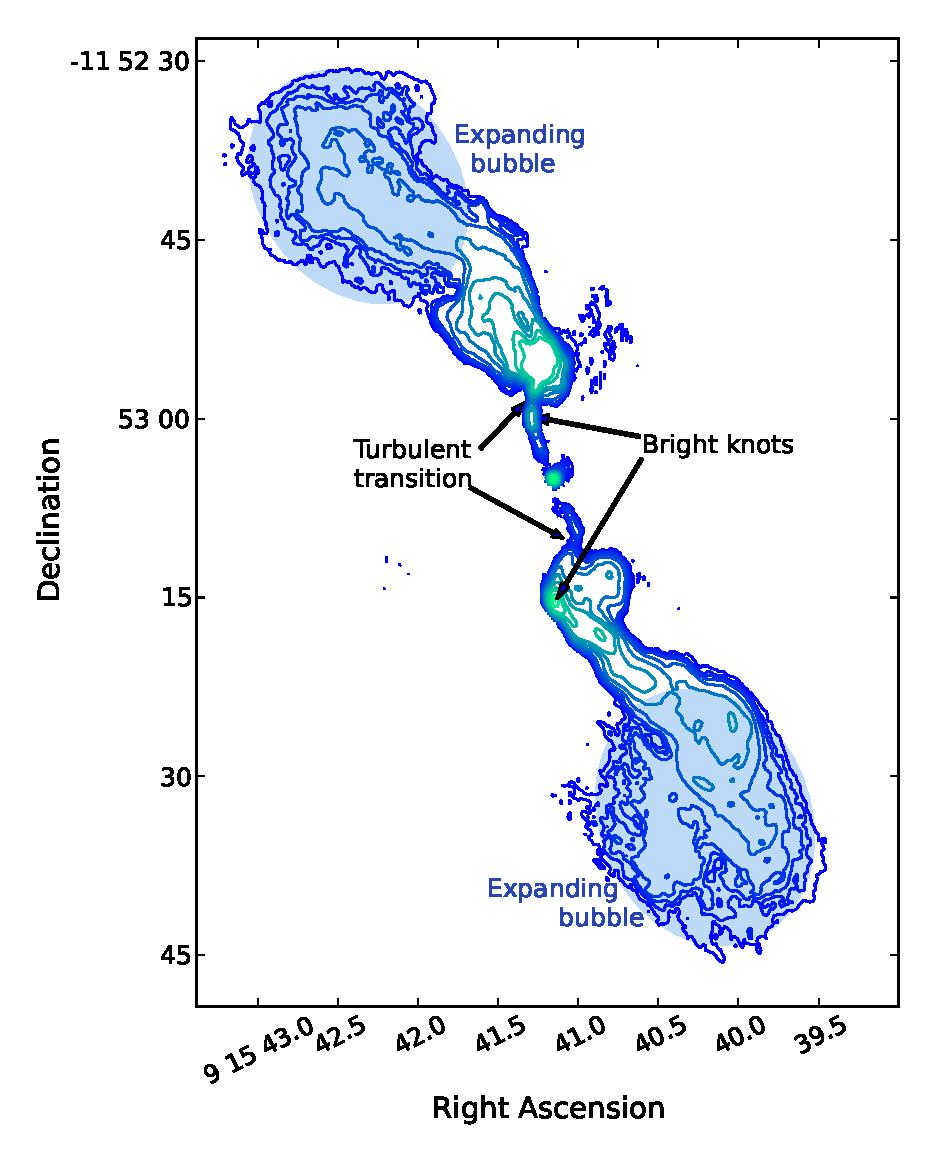
\includegraphics[width=10cm]{taylor.eps}
\caption{ Radio intensity map of Hydra~A at 4.635 GHz. This figure is almost identical to Fig. 1 in \citet{taylor90}. Contour levels are at 1.5, 2.7, 3.7, 5.1, 10, 21, 37, 51, 103, 154, 311, and 466 mJy arcsec$^{-2}$. 
The elliptical areas outline the approximate volume of the corresponding X-ray A and B cavities and are used to estimate the contribution to the jet kinetic power. }
\label{taylor}
\end{figure*}

%\textbf{(b)} Zoom-in of the top rectangular region in a) showing the bright knots in the northern jet. Contours are at 1.5, 2.7, 3.7, 5.1, 6.3, 7.5, 8.8, 10, 21, 37, 51, 72, 90, 103, 154, 311, and 466 mJy arcsec$^{-2}$. \textbf{(c)} Zoom-in of the bottom rectangular region in a) showing the bright knots in the southern jet. Contours are at 1.5, 2.0, 2.2, 2.7, 3.7, 5.1, 5.5, 6.0, 6.3, 6.8, 7.5, 8.8, 10, 21, 37, 51,  72, 90, 103, 154, 311, and 466 mJy arcsec$^{-2}$.



%%%%%%%%%%%%%%%%%%%%
%
% Jet Power from a Shock Model
%
%%%%%%%%%%%%%%%%%%%%
\subsection{Jet power based on a model for the outer shock}\label{s:powsh}

\citet{nulsen05} focused on the outer shock evident in the X-ray image and used a spherically symmetric hydrodynamic model of a point explosion in an initially isothermal and hydrostatic environment to produce theoretical X-ray surface brightness profiles for Hydra~A. Their best fit to the observed X-ray brightness profile gives a shock age $\sim 1.4 \times 10^8 \, \rm Myr$ and an explosion energy $\sim 10^{61} \, \rm erg$. The estimated power of the outburst is $\sim 2 \times 10^{45} \, \rm erg \, s^{-1}$. On the basis of this model, I would associate $10^{45} \> \rm erg \> s^{-1}$ with each jet.

%%%%%%%%%%%%%%%%%%%%
%
% Jet Power from X-ray data
%
%%%%%%%%%%%%%%%%%%%%
\subsection{Jet power based on X-ray cavities}\label{s:powx}

\citet{wise07} used the observations of three pairs of X-ray cavities revealed in \textit{Chandra} images to estimate the power of the Hydra~A jets. The inner cavities A and B correspond to the 4.6~GHz radio lobes \citep{mcnamara00}, the cavities C and D correspond to the middle lobe in the 1.4 GHz radio image \citep{lane04} and the outer cavities E and F correspond to the outer lobes in the 330 MHz image \citep{wise07}. Wise et al. consider that the three cavities on each side are interconnected and use the sum of the enthalpies, $h_{\rm tot}$
\begin{equation}
h_\mathrm{tot}=\gamma p_{\rm lobe}V_{\rm lobe}/(\gamma -1)
\end{equation}
where $\gamma$ is the polytropic index, $p_{\rm lobe}$ is the pressure of the lobe and $V$ is the volume of the cavity, in all cavities to calculate a total outburst energy. From this, the combined jet power is calculated, $P_\mathrm{jet}=4 p_{\rm lobe} V/t_{\rm cav}$, where $t_{\rm cav}$ is the age of each cavity. The average of three different cavity age estimates was used: the time required for the X-ray cavity to reach its present position if moving at the sound speed, the refilling time of the X-ray cavity, and the time required for the X-ray cavity to rise buoyantly to the present position. Assuming pressure equilibrium of the lobes with the atmosphere they obtained powers for the inner and middle lobes of $\sim 2 \times 10^{44} \> \rm erg \> s^{-1}$ and for the outer lobes, $\sim 6 \times 10^{44} \> \rm erg \> s^{-1}$, which gives a combined jet power $\sim 2 \times 10^{45} \> \rm erg \> s^{-1}$. 

The authors find that a power of $1\times10^{45}$ erg s $^{-1}$ for the northern jet is consistent with the supposition that the jet is still filling the outermost of the X-ray cavities at $\sim200$ kpc (the corresponding radio lobe is visible at 330 Mhz) and driving the large-scale shock. An independent estimate of the jet power from the expansion rate of the outermost cavity, assuming a self-similar evolution of the radius of the cavity wall and the large scale shock agrees with their first estimate to within a factor of 2. This value of the jet power $1\times10^{45}$ erg s $^{-1}$ is also consistent with the estimate of the jet power obtained by \citet{nulsen05} noted above. 

\begin{table}
\caption{Parameters for the determination of the lobe minimum energy.} 
\centering
\begin{tabular}{l c c}
 \hline  \hline
 Parameter & Value \\
 \hline 
 Electron spectral index, $a$  &  2.4 \\
 Lorentz factor lower cutoff, $\gamma_1$   &  100                       \\ 
 Lorentz factor upper cutoff, $\gamma_2$ &   10$^6$ \\  
 Central surface brightness, $I_{\nu}$       & 10 mJy arcsec$^{-2}$	 \\ 
 Plasma depth, $L$    & 20 kpc (northern lobe) \\ 
                          & 22 kpc (southern lobe) \\ \hline
\end{tabular}
\label{radio_data}
\end{table}

%%%%%%%%%%%%%%%%%%%%%%%%%


%%%%%%%%%%%%%%%%%%%%
%
% Jet Power from Radio Data
%
%%%%%%%%%%%%%%%%%%%%
%\subsection{Estimates of the power associated with cavities A and B using radio data}\label{s:powr}
\subsection{Estimates of the jet power from synchrotron minimum energy}\label{s:powr}


I revisit the calculation of the cavity powers of the two innermost cavities \citep[see][]{wise07} by using the synchrotron minimum energy estimate for the pressure and synchrotron ages of the lobes. The main difference between this method and that using the X-ray cavities is that the former introduces a strong dependence of the lobe pressure on the particle content of the lobe, whereas the X-ray cavity pressure only depends weakly on the particle content through the adiabatic index. 

The work by \citet{croston05a} on the lobes of classical double (FRII) radio galaxies shows that using a synchrotron minimum energy estimate is a feasible approach. However, since Hydra~A is an FRI source this requires further justification. \citet{croston05a} used observations of the inverse Compton emission in their sample to show that the lobes are close to equipartition when the inverse ratio of energy in relativistic electrons/positrons to that of ``other'' particles, $k=0$. They use this fact to rule out an energetic relativistic proton component since the existence of such a component would imply that the magnetic field is in equipartition with the relativistic electrons only. While the authors did not state this directly, their argument can also be used to exclude an energetic thermal component. This is evident for powerful FRII sources, for which we do not expect much entrainment to occur. However, I argue that the turbulent processes leading to equipartition are independent of the plasma composition and that in the case where the plasma has a substantial thermal content these processes also lead to a minimum energy state between \emph{all} particles and the magnetic field. This conclusion is supported by the work of \citet{birzan08} discussed below.     

I have approximated the shapes of the lobes with ellipsoidal volumes as shown by the shaded elliptical regions in Fig.~\ref{taylor}a; the plasma depth is taken to be equal to the minor axis, $L$. The lobe centres are located at $\sim 30$~kpc from the core. Let $I_\nu$ be the central surface brightness of each lobe, where $\nu=4.6$ GHz is the frequency of the \citet{taylor90} observations. Let $m_{\rm{e}}$ be the electron mass, $e$ the elementary charge, $a$ the electron index, $\alpha=(a-1)/2$ the spectral index, and $\gamma_1$ and $\gamma_2$ the lower and upper cutoff Lorentz factors, respectively. Then, the minimum energy magnetic field (in Gauss) \citep[e.g][]{bicknell13a} of the synchrotron radiating plasma is given by: 

\begin{equation}
B_{\rm{min,E}} = \frac{m_{\rm{e}} c}{e}\left[ \frac{a+1}{2}(1+k)C^{-1}(a)\frac{c}{m_{\rm{e}}}f(a,\gamma_1, \gamma_2)\frac{I_{\nu}\nu^{\alpha}}{L} \right]^{\frac{2}{a+5}}\;,
\label{e:bmin}
\end{equation}
where 
\begin{equation}
f(a, \gamma_1, \gamma_2) = (a-2)^{-1} \gamma_1^{-(a-2)} \left [ 1 - \left( \frac{\gamma_2}{\gamma_1}\right)^{-(a-2)}\right]\:,
\end{equation}
and 
\begin{eqnarray}
C(a) &=& 3^{a/2}2^{-(a+7)/2}\pi^{-(a+3)/2} \nonumber  \\
&& \times  \frac{\Gamma\left(\frac{a}{4}+\frac{19}{12}\right)\Gamma\left(\frac{a}{4}-\frac{1}{12}\right)}{a+1} \> 
\frac{\sqrt{\pi}}{2}\frac{\Gamma\left(\frac{5+a}{4}\right)}{\Gamma \left(\frac{7+a}{4}\right)}\;.\label{eq:ca}
\end{eqnarray}
In Eqn.~\eqref{eq:ca} $\Gamma$ is the Gamma-function. Values adopted for $a$, $\gamma_1$, $\gamma_2$, $I_{\nu}$, and $L$ are shown in Table \ref{radio_data}. I choose a spectral index $\alpha\approx0.7$ (hence $a=2.4$), which is representative of the low frequency spectral index of the radio emission \citep{cotton09}.
I choose a lower Lorentz cutoff $\gamma_1=100$, in view of numerous studies of radio galaxies finding $\gamma\sim100-10^3$  \citep{carilli91,  hardcastle01, godfrey09}. Also, $\gamma_2\approx10^6$, since this corresponds to emission frequencies well above the microwave range. Minimum energy estimates are insensitive to $\gamma_2$ and only weakly dependent on $\gamma_1$.

The minimum total (particles + field) energy density of the lobe is given by 
\begin{equation}
\varepsilon_{\rm{tot}} = \varepsilon_{\rm p} + \frac {B_{\rm min,E }^2}{8 \pi} = \frac{a+5}{a+1}\frac{B_{\rm{min,E}}^2}{8 \pi}\;,
\end{equation}
and the total pressure of the lobe corresponding to the minimum total energy density is
\begin{equation}
p_{\rm{tot}}=\frac{1}{3}\varepsilon_\text{e}(1+k)+\frac{B_\text{min,E}^2}{8 \pi}\:.
\label{total_pressure}
\end{equation}
The major uncertainty in this calculation arises from the lack of observational constraints on the parameter $k$. The value of $k$ determines whether the lobe (in equipartition) is over-pressured or under-pressured with respect to the environment, and later in this section I discuss the range of values for $k$ applicable to the Hydra~A radio lobes. Estimates of $B_{\rm{min,E}}$ and $p_{\rm{tot}}$ are given in Table \ref{minimum_energy} for three values of $k$. 

I estimate the age of the source from the curvature in the spectrum derived by \citet{cotton09} who showed that the spectra of the inner lobes steepen for frequencies $\geq 300 \> \rm MHz$. Let $B=B_\mathrm{min,E}$ be the minimum energy magnetic field and $\nu_{\rm{b}} \approx 300 \> \rm MHz$ be the break frequency, then the synchrotron age of the source is 
\begin{equation}
t_{\rm{rad}} \approx \frac{3^{5/2}}{8 {\pi}^{1/2}} \left(\frac{m_e^3 c^5}{e^3}\right)^{1/2} B^{-3/2}\nu_{\rm{b}}^{-1/2}\:.
\end{equation}
Hence, the power associated with each of the inner cavities is 
\begin{equation}
P_{\rm cav} = \frac{\gamma}{(\gamma -1)} \frac{p_{\rm lobe} V_{\rm lobe}}{t_{\rm rad}}.
\label{p_cav}
\end{equation}
I use the total pressure $p_{\rm{tot}}$ for minimum energy conditions as the lobe pressure. Values of $P_{\rm{cav}}$ for different values of $k$ are given in Table \ref{minimum_energy}.



%%%%%%%%%%%%%%%%%%%%%%%
%
%	Table: jet_parameters
%
%%%%%%%%%%%%%%%%%%%%%%% 


\begin{table*}
\caption{Parameters calculated for three values of $k$ using synchrotron minimum energy for both lobes of Hydra A. }
\label{minimum_energy}
\centering
\begin{threeparttable}
\begin{tabular}{*{7}{c}}
\hline \hline
   $k$ & $B_{\rm{min,E}}$  & $\varepsilon_{\rm{tot}}$  & $p_{\rm{tot}}$ &  $p_{\rm{tot}}/p_{\rm{a}}$ & $P_{\rm{cav}}$ & $t_{\rm{rad}}$    \\
       & (10$^{-6}$ Gauss)  & ($10^{-10}$ erg cm$^{-3}$) &  ($10^{-10}$ dyne cm${^{-1}}$) & & ($10^{44}$ erg s$^{-1}$) & (Myr)  \\ 
             \multicolumn{7}{c}{Northern Lobe} \\ \hline
%           &  \multicolumn{7}{c}{\it Electrons + non-relativistic particles} \\ 
  0 & 22 & 0.4 & 0.3  & 0.2 & 0.1 & 49  \\ 
  10 & 42 & 1.5 & 1.2 & 0.9 &  1.8 &  18 \\ 
  100 & 76 & 4.9 &  3.9 & 3.0 & 14.5  & 7  \\
%           &  \multicolumn{7}{c}{\it Electrons + relativistic particles} \\ 
%  0 & 22 & 0.4 & 0.3  & 0.1 &  0.1 & 32 & 0.1 & 49  \\ 
%  10 & 42 & 1.5 & 1.2 & 0.6 &  1.0 & 14  & 1.3 & 18 \\ 
%  100 & 76 & 4.9 &  3.9 & 2.0 &  6.0 & 8 & 15.4 & 7  \\
  \hline
   \multicolumn{7}{c}{Southern Lobe} \\ \hline
       0 &  21 & 0.4 & 0.3 & 0.2 &  0.1  & 51 \\
       10 & 40 & 1.4 & 1.1 &  0.9 &  2.0 & 19 \\ 
       100 & 73 & 4.6 & 3.7 & 3.0 &  16.3   & 8 \\
\hline
\end{tabular}
\end{threeparttable}
\end{table*}


Table \ref{minimum_energy} shows, for both the northern and southern lobes, the estimation of the minimum energy magnetic field, $B_{\rm{min,E}}$, the total energy density $\varepsilon_{\rm tot}$, the total pressure of the lobe, $p_{\rm{tot}}$, the ratio between the total lobe pressure and the atmospheric pressure $p_{\rm{tot}}/p_{\rm{a}}$, the cavity power for $\gamma = 4/3$, and the radiative ages of the lobes for values of the parameter $k=0, \ 10 \rm \ and \ 100$.

For the same value of $k$, the cavity powers of the northern and southern lobes are comparable. Moreover, for $k=10$ the lobes are in approximate pressure equilibrium with the atmosphere and the cavity powers ($1.8 \times 10^{44}$ and $2.0\times 10^{44} \> \rm ergs \> s^{-1}$ respectively) agree with the \citet{wise07} estimates of $2.1\times 10^{44} \> \rm ergs \> s^{-1}$ and $2.0\times 10^{44} \> \rm ergs \> s^{-1}$ respectively. For $k=0$ the lobes appear to be significantly under-pressured and for $k=100$ significantly over-pressured.

This high value of $k$, i.e., energy dominated by the heavy particles, is  supported by a recent study performed by \citep{birzan08}. They estimate $k$ for a group of galaxies including Hydra A assuming pressure equilibrium between the radio lobe and the atmosphere. For the 1.4GHz inner lobe of Hydra A they obtained a value of $k\approx13$. In their study of the inverse-Compton X-ray emission of the outer lobe of Hydra A \citet{hardcastle10} estimates a moderate value of $k=17 - 23$. 

The major uncertainty associated with these radio-based estimates of the cavity power is that there is no direct estimate of the lobe pressure and I have assumed that the lobe pressure is determined by the total pressure of the lobe when the lobe is in its minimum energy state. This assumption gives a lower limit of the lobe energy, and hence a lower limit on the cavity power.


The estimation of the power associated with the inner radio lobes and the power of the corresponding X-ray cavities given in \S~\ref{s:powx} for a nearly pressure equilibrium situation are consistent. This indicates the total jet power obtained by summing the powers of all X-ray cavities presented presented by \citet{wise07} is reliable and provides a sound basis for numerical models of Hydra A.  
I therefore adopt a jet power of $10^{45} \> \rm erg \> s^{-1}$ as our value in the simulations presented in \S~\ref{s:sims}. 

% with the cavity power estimates for the northern and southern lobes respectively. 
%This indicates that the result for the total jet power from the summation of all cavity powers, obtained by \citet{wise07} is reliable and provides a sound basis for numerical models of Hydra A. 

%%%%%%%%%%%%%%%%%%%%%%%%%%%%%%%%%%%%%%%%%%%%
%
%					Cluster Environment
%
%%%%%%%%%%%%%%%%%%%%%%%%%%%%%%%%%%%%%%%%%%%%
\section{Cluster Environment} \label{s:cluster}
 

\begin{figure}
\centering
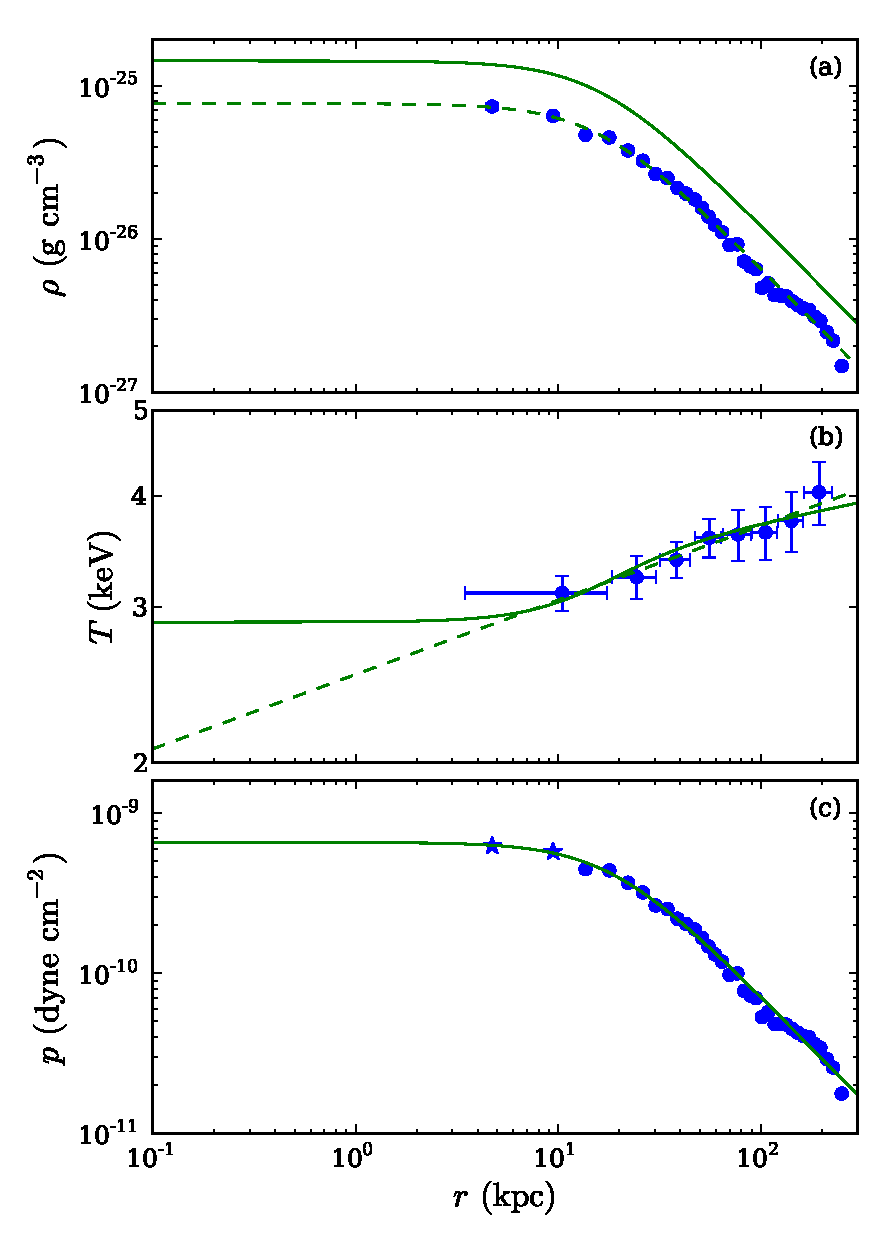
\includegraphics[width=130mm]{ICM.eps}
\caption{Radial thermodynamic profiles for the Hydra A galaxy cluster. \textbf{(a)} Electron density (data points and dashed line), and corresponding total particle density (solid line) assuming a fully ionized plasma; Error bars are smaller than the points. \textbf{(b)} Electron temperature (data points and dashed line) and the temperature profile obtained from the total particle density and the pressure profiles (solid line); \textbf{(c)} Total pressure. The points in (a) and (b) are data for the electron density and electron temperature, respectively, obtained by \citet{david01} from X-ray observations of the Hydra A atmosphere. The dashed curves are fits to the data points using Eqn~\ref{density_profile} for (a) and a power-law for (b). The points in (c) were calculated from the density data points and the temperature fit. The stars represent the additional data points that I obtained through this method inside of 10 kpc. These two data points are important in constraining the profiles in the innermost region. The line in (c) is a fit to the data with Eqn.~\eqref{pressure_profile}.
Finally the temperature profile (solid line in panel b)) is obtained from the total particle density and the pressure profile. \newline
(A colour version of this figure is available in the online journal)}
\label{profiles}
\end{figure}


\begin{table}
\caption{Atmosphere profile parameters. Fits to data by \citet{david01} and extrapolation to $r<10$ kpc.} 
\centering
\begin{tabular}{r c c}
 \hline\hline
 & Parameter & Best fit value \\
 \hline
 \multirow{3}{*}{Density profile} & $r_{\rho 0}$ &  15.94 kpc \\
 & $\rho_0$     &  $1.49\times 10^{-25}$ g cm$^{-3}$ \\
 & $\alpha_{\rho}$ & 0.67  \\  
 \hline
 \multirow{2}{*}{Temperature profile} & $a_T$   & 5.66     \\
 & $b_T$   & $8.4\times10^{-2}$ \\
 \hline
 \multirow{3}{*}{Pressure profile} & $r_{p0}$  & 18.21 kpc	 \\
 & $p_0$     &	$6.58 \times 10^{-10}$ dyne cm$^{-2}$ \\
 & $\alpha_{p}$ & 0.65  \\
 \hline
\end{tabular}
\label{halo parameters}
\end{table}


In order to construct definitive simulations of the inner jet propagation, I require knowledge of the distribution of the ambient density and pressure on a 10~kpc scale. In this section I present useful analytical fits for the density, temperature, and pressure in the cluster environment, which I use to estimate the pressure and density in the inner 10 kpc.

I assume that Hydra A's atmosphere prior to the passage of the jet is hydrostatic, following a spherically-symmetric density distribution of the form
\begin{equation}
\rho(r) = \frac{\rho_0}{(1+r^2/r_{\rho0}^2)^{\alpha_{\rho}}}\:.
\label{density_profile}
\end{equation}
$\rho_0$, $r_{\rho0}$, and $\alpha_{\rho}$ are determined through a least-squares fit of the function given in Eqn.~\eqref{density_profile} to the models for the cluster density inferred from the X-ray surface brightness by \citet{david01}. The data and the fitted density profile are shown in Fig.~\ref{profiles} a). The pressure distribution of the atmosphere depends on the temperature distribution through 
\begin{equation}
p = \rho k_B T/\mu m
\end{equation}
 where $k_B$ is Boltzmann's constant, $\mu$ is the molecular weight and $m$ is the atomic mass unit. However, there is no observational data for the temperature inside of 10 kpc. I therefore use a power law temperature fit, $\log T = a_T+b_T\log r$, as shown in Fig.~\ref{profiles} b), to the \citet{david01} data and the density profile given by Eqn.~\eqref{density_profile} to obtain corresponding pressure values for two additional points within a radius of 10 kpc; these are distinguished from the other data points by the star-shaped symbols in Fig.~\ref{pressure_profile} c). The two additional extrapolated data points are important in constraining the shape of the flattening pressure profile toward the core of the galaxy. I adopt the following analytic expression for the pressure profile of the ICM
\begin{equation}
p(r) = \frac{p_0}{(1+r^2/r_{p0}^2)^{\alpha_p}}\:.
\label{pressure_profile}
\end{equation}
A least squares fit to the pressure data points is used to obtain the parameters  $p_0$, $r_{p0}$, and $\alpha_p$.  
 We then obtain the final temperature fit (solid line in panel b)) using the total particle density (solid line in panel a)) and the pressure profile (solid line in panel c)). 
 The best-fit parameters for the fits to the density, temperature, and pressure data are summarised in Table \ref{halo parameters}. 

For a hydrostatic environment I now have a gravitational acceleration profile
\begin{equation}
g(r) = - \frac {1}{\rho} \frac {dp}{dr} =  -2\alpha_p \frac{p_0}{\rho_0} \frac{r}{r_{p0}}\frac{(1+r^2/r_{\rho0}^2)^{\alpha_{\rho}}}{(1+r^2/r_{p0}^2)^{1+\alpha_p}}\:.
\end{equation}

